\documentclass[../main.tex]{subfiles}

\begin{document}
\chapter{Lecture 4 - 07-04-2020}

We spoke about Knn classifier with voronoi diagram

$$
\hat{\ell}(\hnn) = 0 \qquad \forall \, \textit{Traning set}
$$
\\
$\hnn$ predictor needs to store entire dataset.
\\
\section{Computing $\hnn$}
Computing $\hnn(x)$ requires computing distances between x and points in the traning set.
\\
$$
\Theta(d) \quad \textit{time for each distance}
$$

NN $\rightarrow$ 1-NN\\
We can generalise NN in K-NN with $k = 1,3,5,7$ so odd $K$ \\
$\hknn(x)$ = label corresponding to the majority of labels of the k closet point to
x in the training set.\\\\
How big could $K$ be if i have $n$ point?\\
I look at the $k$ closest point\\
When $k = m$?\\
The majority, will be a constant classifier
$\hknn$ is constant and corresponds to the majority of training labels\\
Training error is always 0 for $\hnn$, while for $\hknn$ will be typically $>0$, with $k >
1$\\
Image: one dimensional classifier and training set is repeated.
Is the plot of 1-NN classifier.\\
Positive and negative.
$K = 1$ error is 0.\\
In the second line we switch to $k =3$. Second point doesn’t switch and third will
be classify to positive and we have training mistake.\\
Switches corresponds to border of voronoi partition.
$$\knn \qquad \textit{For multiclass classification}$$
$$
(|Y| > 2 ) \qquad \textit{for regression } Y\equiv \barra{R}
$$
\\
Average of labels of $K$ neighbours $\rightarrow$ i will get a number with prediction.
\\
I can weight average by distance
\\
You can vary this algorithm as you want.\\\\
Let’s go back to Binary classification.\\
The $k$ parameter is the effect of making the structure of classifier more
complex and less complex for small value of $k$.\\\\
\begin{figure}[h]
    \centering
    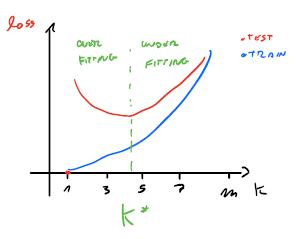
\includegraphics[width=0.4\linewidth]{../img/lez4-img1.JPG}
    \caption{Example of domain of $\knn$}
    %\label{fig:}
\end{figure}\\
Fix training set and test set\\
Accury as oppose to the error
\\\\
Show a plot. Training error is 0 at $k = 0$.\\
As i go further training error is higher and test error goes down. At some point
after which training and set met and then after that training and test error goes
up (accuracy goes down).\\
If i run algorithm is going to be overfitting: training error and test error is high and also underfitting since testing and training are close and both high.
Trade off point is the point in $x = 23$ (more or less).\\
There are some heuristic to run NN algorithm without value of $k$.
\\\\
\textbf{History}
\begin{itemize}
\item $\knn$: from 1960 $\rightarrow$ $X \equiv \barra{R}^d$
\item Tree predictor: from 1980
\\
\end{itemize}

\section{Tree Predictor}
If a give you data not welled defined in a Euclidean space.
\\
$X = X_1 \cdot x \cdot ... \cdot X_d \cdot x$ \qquad Medical Record
\\
$X_1 = \{Male, Female\}$\\
$X_2 = \{Yes, No\}$
\\
so we have different data
\\\\
I want to avoid comparing $x_i$ with $x_j$,  $i\neq j $\\
so comparing different feature and we want to compare each feature with
each self. I don’t want to mix them up.\\
We can use a tree!
\begin{figure}[h]
    \centering
    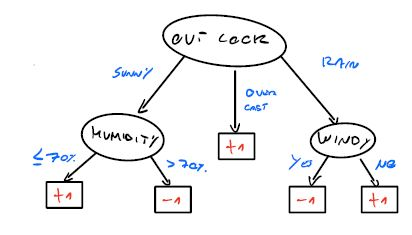
\includegraphics[width=0.5\linewidth]{../img/lez4-img2.JPG}
    \caption{Example of domain of $\knn$}
    %\label{fig:}
\end{figure}\\
\\
I have 3 features:
\begin{itemize}
\item outlook  $= \{sunny, overcast, rain\}$
\item humidity $= \{[0,100]\}$
\item windy $ = \{yes,no\}$
\end{itemize}
Tree is a natural way of doing decision and abstraction of decision process of
one person. It is a good way to deal with categorical variables.\\
What kind of tree we are talking about?\\
Tree has inner node and leaves. Leaves are associated with labels $(Y)$ and
inner nodes are associated with test.
\begin{figure}[h]
    \centering
    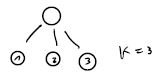
\includegraphics[width=0.3\linewidth]{../img/lez4-img3.JPG}
    \caption{Example of domain of $\knn$}
    %\label{fig:}
\end{figure}\\
\begin{itemize}
\item Inner node $\rightarrow$ test
\item Leaves $\rightarrow$ label in Y
\end{itemize}
Test if a function $f$ (NOT A PREDICTOR!) \\
Test $ \qquad f_i \, X_i \rightarrow \{1,...,k\}$
\\ where $k$ is the number of children (inner node) to which test is assigned
\\
In a tree predictor we have:
\begin{itemize}
\item Root node
\item Children are ordered(i know the order of each branch that come out from the node)
\end{itemize}
$$
X = \{Sunny, 50\%, No \} \quad \rightarrow \quad \textit{are the parameters for } \{outlook. humidity, windy \} 
$$
\\
$
f_i = 
\begin{cases} 
1, & \mbox{if } x_2 \in [30 \%,60 \% ] 
\\ 
2, & \mbox{if } otherwise \end{cases}
$
\\ where the numbers 1 and 2 are the children
\\
A test is partitioning the range of values of a certain attribute in a number of
elements equal to number of children of of the node to which the test is
assigned.
\\
$h_T(x)$ is always the label of a leaf of T\\
This leaf is the leaf to which $x$ is \textbf{routed}
\\
Data space for this problem (outlook,..) is partitioned in the leaves of the tree.
It won’t be like voronoi graph.
How do I build a tree given a training set?
How do i learn a tree predictor given a training set?
\begin{itemize}
\item Decide tree structure (how • many node, leaves ecc..)
\item Decide test on inner nodes
\item Decide labels on leaves
\end{itemize}
We have to do this all together and process will be more dynamic.
For simplicity binary classification and fix two children for each inner node.\\\\
$ Y = \{-1, +1 \}$
\\ $2$ children for each inner node
\\\\
What's the simplest way?\\
Initial tree and correspond to a costant classifier
\\
\begin{figure}[h]
    \centering
    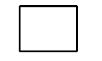
\includegraphics[width=0.2\linewidth]{../img/lez4-img4.JPG}
    \caption{Example of domain of $\knn$}
    %\label{fig:}
\end{figure}\\
\textbf{Majority of all example}
\\
\begin{figure}[h]
    \centering
    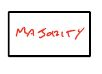
\includegraphics[width=0.2\linewidth]{../img/lez4-img5.JPG}
    \caption{Example of domain of $\knn$}
    %\label{fig:}
\end{figure}\\
$(x_1, y_1) ... (x_m, y_m)$ \\
$ x_t \in X$ \qquad $ y_t \in \{-1,+1\}$\\
Training set $S = \{ (x,y) \in S$, x is routed to $\ell\}$\\
$S_{\ell}^+$ 
\\
\begin{figure}[h]
    \centering
    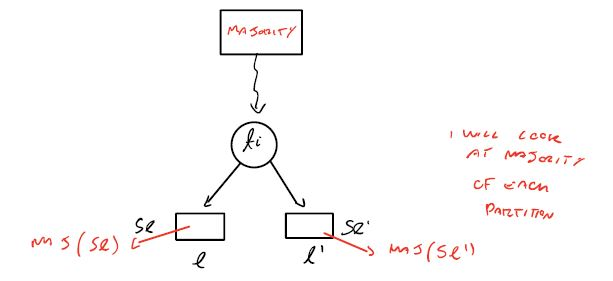
\includegraphics[width=0.8\linewidth]{../img/lez4-img6.JPG}
    \caption{Example of domain of $\knn$}
    %\label{fig:}
\end{figure}\\
$ S_{\ell}$ and $ S’_{\ell}$ are given by the result of the test, not the labels  and $\ell$ and $\ell'$.\\
\begin{figure}[h]
    \centering
    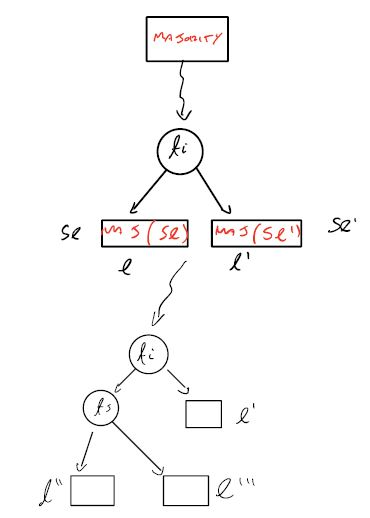
\includegraphics[width=0.7\linewidth]{../img/lez4-img7.JPG}
    \caption{Example of domain of $\knn$}
    %\label{fig:}
\end{figure}
\end{document}